\documentclass[11pt,fleqn]{article}

\setlength {\topmargin} {-.15in}
\setlength {\textheight} {8.6in}

\usepackage{amsmath}
\usepackage{amssymb}
\usepackage{color}
\usepackage{tikz}
\usetikzlibrary{automata,positioning,arrows}
\usepackage{diagbox}
\usepackage{stackrel}
\begin{document}


\textbf{Exercise 1.4.8} Write a program to determine the number pairs of values in an input file that
are equal. If your first try is quadratic, think again and use Arrays.sort() to develop
a linearithmic solution.\\

\textbf{Solution:}
\begin{itemize}
	\item Since we want a linearithmic solution, like we can use Binary search due to $log_2N$ complexity while iterating through the array to search for the next element that isn't the same as previous element..
	\item If the array is not sorted, then sort the array using $Array.sort()$
	\item Go through the array of elements.
	\item Use binary search to find first and last instance of an element.
	\item subtract the indices and then add 1 since our indices start at index 0.
	\item Check for the next element in array, if it is an element we already saw previously, then ignore it. If found a new element, then again repeat above steps using BinSearch to find first and last occurences. Basically, do this for each unique element.
	\item ie; 1,2,2,2,2,3
	
\end{itemize}

\newpage
Pseudocode below:
\begin{center}
	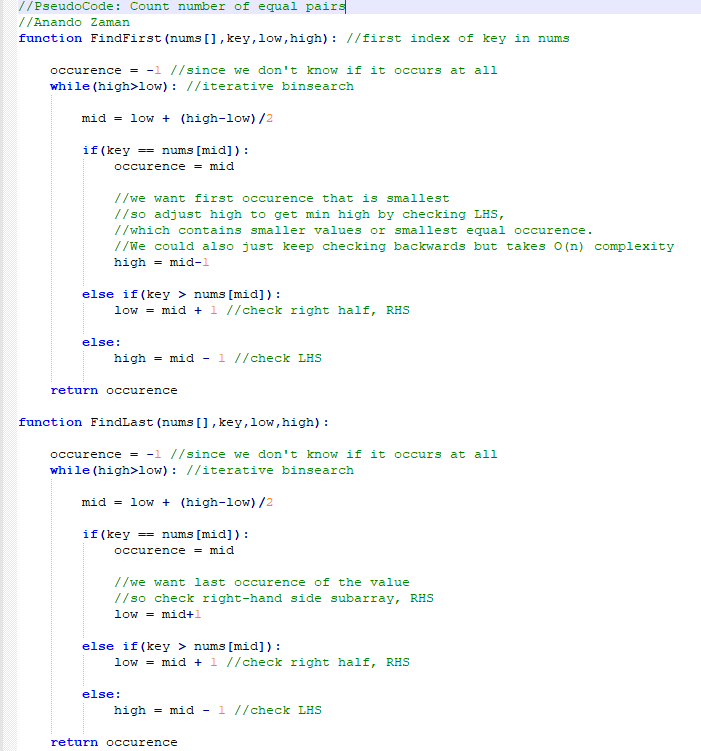
\includegraphics[scale = 1]{1.4.8.png}
	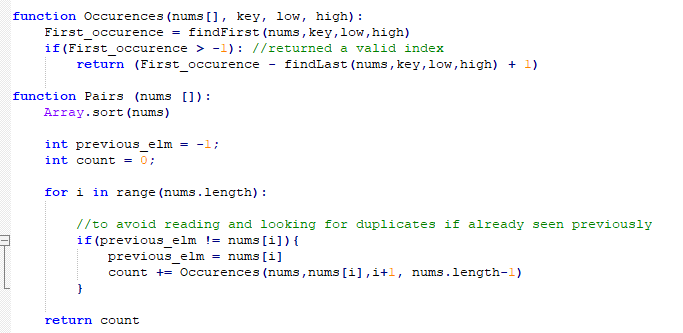
\includegraphics[scale = 1]{1.4.8-1.png}
	\end{center}

\end{document}
